\documentclass[man,floatsintext]{apa6}
\usepackage[nodoi]{apacite}
\usepackage{graphicx}
\usepackage[american]{babel}
\usepackage{amsmath}
\usepackage{enumitem}
\usepackage[section]{placeins}
\usepackage{caption}
\usepackage{subcaption}

\title{Preschoolers flexibly adapt to linguistic input in a noisy channel}
\author{Daniel Yurovsky$^1$, Sarah Case$^2$, and Michael C. Frank$^2$}
\affiliation{$^1$Department of Psychology, University of Chicago\\
    $^2$Department of Psychology, Stanford University}
\shorttitle{Noisy Channel Processing in Children}
\leftheader{Yurovsky, Case, \& Frank}


\abstract{
Because linguistic communication is inherently noisy and uncertain, adult language comprehenders integrate bottom-up cues from speech perception with top-down expectations about what speakers are likely to say. Further, in line with the predictions of ideal observer models, comprehenders flexibly adapt how much they rely on these two kinds of cues in proportion to their changing reliability. Do children also show evidence of flexible, expectation-based language comprehension? We presented preschoolers with ambiguous utterances that afforded two different interpretations, depending on whether they privileged perceptual input or top-down expectations. Across three experiments, we manipulated the reliability of both their perceptual input and their expectations about the speaker's intended meaning. As predicted by noisy channel models of speech processing, 4- and 5-year-old---but perhaps not younger---children flexibly adjusted their interpretations as cues changed in reliability.}

\keywords{Language processing, noisy channel, cognitive development}

\authornote{Please address correspondence to:

\vspace{12 pt}
Daniel Yurovsky

Department of Psychology

University of Chicago

5848 S University Avenue

Chicago IL, 60637

\vspace{12 pt}
Email: yurovsky@uchicago.edu

\vspace{24 pt}}

\begin{document}
\maketitle

Imagine Bob hears Alice say ``I had carrots and bees for dinner.'' Perhaps she visited an exotic restaurant, and he should ask how they tasted. Or perhaps he misheard her or she misspoke---she actually ate \emph{peas}. To interpret Alice's utterance, Bob has to integrate perceptual information from her speech with his expectations about what words usually go with ``carrots'' and ``dinner'' and what foods people usually eat. Modern statistical language processing systems use a body of theory based on this idea---that language is a \emph{noisy channel}, and that Bob can correct for perceptual errors using linguistic expectations about what Alice was likely trying to say \cite{jelinek1976, shannon1948}.

Noisy channel principles provide a powerful framework for explaining how people process language in complex and uncertain real-time communicative situations \cite{clayards2008, levy2008, jaeger2010}. On this view of language, comprehenders integrate prior expectations with perceptual data probabilistically, weighting each according to its reliability \cite{ernst2002, jacobs1999}. In one demonstration of such integration, \citeA{gibson2013} presented participants with semantically implausible sentences (e.g., ``The mother gave the candle the daughter''), which could have been produced by small typographical errors in otherwise much more plausible sentences (``The mother gave the candle \emph{to} the daughter''). Adults corrected these errors, and critically did so more often when they thought the communicative channel was noisy (and hence the perceptual signal was unreliable). Conversely, adults corrected these errors less often when they thought they were in a ``silly'' context where many other sentences were similarly implausible.

Do children also process language in the same flexible, expectation-based way? Toddlers use speakers' social and pragmatic cues to determine their intended referent in otherwise ambiguous situations \cite{carpenter1998, clark2009}. They also use acoustic cues like speaker identity and linguistic cues like grammatical gender \cite{lew-williams2007, creel2012}. However, these successes have been shown only when all cues point to the same meaning. When top-down and bottom-up cues conflict, preschoolers often over-weigh, or even attend exclusively to lower-level cues \cite{trueswell1999,snedeker2004}.

Outside of language processing, even older children sometimes fail to combine cues \cite{gori2008,nardini2008,nardini2010}. For example, while adults integrate haptic and visual cues to estimate both size and orientation, 8-year-olds rely exclusively on vision for orientation and haptics for size. Thus, children's successful use of independent information---for example, about high-level speaker expectations\cite{graham2014,matthews2010} or speaker reliability \cite{pasquini2007}---does not their guarantee integration with perceptual uncertainty.

% In fact, in language processing, children sometimes show striking deficits in revising incorrect expectations about meaning in cases where syntax and context compete \cite{trueswell1999,snedeker2013}. But because these failures occur in complex contexts designed to test the development of other abilities, the question remains unanswered. Our current experiments test adaptive, expectation-based integration in the absence of other processing demands.

We created a paradigm to independently manipulate expectations about speaker plausibility and perceptual noise. We introduced preschoolers (and adults) to either a Plausible or Implausible Speaker who initially uttered unambiguously different sentences like ``my cat has three little [kittens/hammers]'' (Figure \ref{fig:exposure}). Participants were then asked to resolve the intended meaning for ambiguous sentences like the ``bees/peas'' example above, which could either be produced by a perceptual error, or could convey implausible content (Figure \ref{fig:test}). If children integrate speaker expectations and channel noise, their interpretations should be a product of both.

% In Experiment 1, we first test this hypothesis by manipulating speaker plausibility. In Experiment 2, we replicate Experiment 1, and cross speaker plausibility with a manipulation of channel noise.

\begin{figure}[tb]
     \centering
        \begin{subfigure}[b]{.4 \textwidth}
            \caption{\label{fig:exposure}}
            
\includegraphics[width=\textwidth]{figures/exposure.pdf}
        \end{subfigure}\quad
        \vspace{12 pt}
        \begin{subfigure}[b]{.4 \textwidth}
           \caption{\label{fig:test}}
           
\includegraphics[width=\textwidth]{figures/testing.pdf}
        \end{subfigure}
    \caption{Example Exposure and Test trials. On Exposure trials, the two pictures and their corresponding referring expressions were highly distinct (e.g. ``my cat has three little [kittens/hammers].'' In contrast, the two pictures on Test trials could be referred to by expressions that contained a single phonological error (e.g. ``I had carrots and [bees/peas] for dinner.'' Children and adults introduced to a speaker who consistently referred to the plausible referent on Exposure trials were more likely to interpret a reference to the implausible picture on Test trials (``bees'') as a reference to the plausible picture (``peas'').}
   \label{fig:stimuli}
\end{figure}

\section{Experiment 1}

\subsection{Method}
\subsubsection{Participants}

Children were recruited at the Bing Nursery School on Stanford's campus. Each child was asked if they would be willing to play a game with the experimenter, and informed that they could stop playing at any time. Children were randomly assigned to speaker conditions, and we collected data until there were at least 20 participants in each condition (similar to other psycholinguistic studies of children \citeNP<e.g.>{trueswell1999, creel2012}). Data from a total of 43 children were collected; children were all between 4 and 6 years old, and approximately half were female. Neither age nor gender distribution varied significantly across conditions (Plausible: 23 children [12 girls], Mean age = 4.6 years [range = 4.0--5.3 years], Implausible: 20 children [10 girls], Mean age = 4.7 years [range = 4.1--5.4 years]).

Adult participants were recruited through Amazon Mechanical Turk. We posted 50 Human Intelligence Tasks (HITs) to be completed only by participants with US IP addresses that each paid 30 cents. A total of 50 HITs were posted, with Speaker condition assigned randomly to each participant. A sample size of 50 was chosen on the basis of the effect size in the child data.

\subsubsection{Stimuli, Design, and Procedure}

Experiment 1 consisted of a series of trials on which participants saw two pictures and heard a sentence referring to one of them. Pictures were constructed from clipart freely available on the internet, and audio was recorded by a female native speaker of English. In order to increase the ambiguity of the spoken utterances, and thus give us more power to detect error-correction, all of the audio recordings were convolved with Brown noise of amplitude $\sim$.6 using the Audacity audio editor and then played back through computer speakers to produce additional distortion. The average signal-to-noise ratio in these recordings was 4.5dB.

Each trial contained one semantically plausible picture and one semantically implausible picture. On Exposure trials, these pictures and their corresponding referring expressions were highly distinct (Figure~\ref{fig:exposure}). In contrast, on Test trials the two pictures corresponded to referring expressions that were only one consonant or vowel apart (Figure~\ref{fig:test}). Each participant saw eight Exposure trials, followed by seven Test trials. The order of these trials within each of these two blocks was randomized across participants, as was the on-screen position of the two pictures on each trial. For participants in the Plausible Speaker condition, the speaker referred to the plausible referent on each of the eight Exposure trials. In contrast, for participants in the Implausible Speaker condition, the speaker referred to the implausible referent on each Exposure trial. In both conditions, the speaker referred to the implausible referent on all seven Test trials.

For all participants, the experiment began with a short introduction to Katie, the speaker who would be referring to pictures for the remainder of the task. After seeing her picture and being introduced to her, participants completed the remaining trials, responding either with the mouse (adults), or by touching one of the pictures on an iPad (children). Audio was presented to children through a set of external computer speakers approximately 2.5 feet away. Adults performed the experiment through Amazon Mechanical Turk, and thus their listening conditions were likely more variable. Adults were instructed by a series of written prompts; children were given instructions by a live experimenter. Three children's responses were coded from video due to a software error. All experiments and analysis code can be found at {\small \tt{dyurovsky.github.io/noisy-kids/}} and all stimuli are available at the linked GitHub repository {\small \tt{github.com/dyurovsky/noisy-kids}}.

\subsection{Results}


In order to validate our manipulation, we first analyze the effect of the speaker on Exposure trials. If participants were attending to the speaker's requests during Exposure trials, those in the Plausible condition should have been more likely to choose the plausible referent (e.g. kittens), and those in the Implausible condition should have been more likely to choose the implausible referent (e.g. hammers). We tested this prediction formally by fitting a mixed-effects logistic regression predicting choice on Exposure trials separately for children and adults ($Exposure \sim condition + (1|subj) + (1|item)$). In this and all other models we report, conditions were dummy coded, and Implausible was treated as the reference category. Random effects for all models were always maximal--random intercepts for subjects and items. As predicted, both children and adults selected the plausible referent more often in the Plausible condition ($\beta_{child} = 4.54$,  $z = 8.28$, $p <.001$, $d = 5.56$; $\beta_{adult} = 9.41$,  $z = 5.83$, $p <.001$, $d = 24.3$). We then fit a model to all of the data, asking whether adults and children were differentially affected by speaker condition ($Exposure \sim condition \cdot age + (1|subj) + (1|item)$). We found significant effects of condition, age group, and their interaction ($\beta_{Plausible} = 9.52$,  $z = 7.87$, $p <.001$,  $\beta_{child} = 1.96$,  $z = 3.33$, $p <.001$; $\beta_{child\: \cdot \: Plausible} = -5$,  $z = -4.12$, $p <.001$). Thus, both children and adults were sensitive to the speaker manipulation during Exposure trials, selecting the appropriate referent whether or not the request was implausible, although adults selected the correct referent more often in both conditions.

\begin{figure}[tb]
\centering
     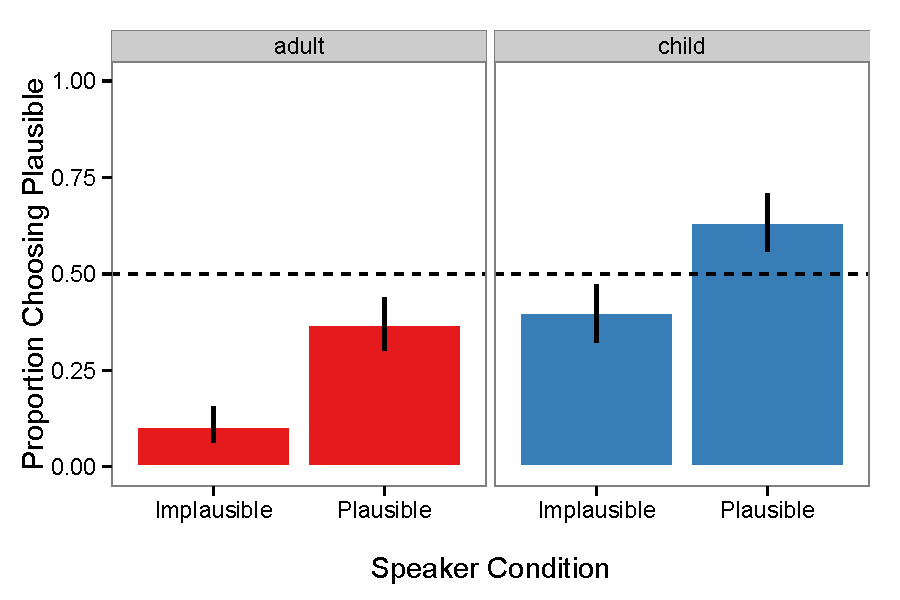
\includegraphics[width=5in]{figures/exp1_results.pdf}
    \caption{Experiment 1 Test trial selections for both children and adults. In line with the predictions of a noisy channel model of language processing, both children and adults were more likely to correct the phonological error during Test trials when they were previously exposed to a Plausible Speaker. Bars show group-averaged proportion of plausible item selection at Test, error bars show 95\% confidence intervals computed by non-parametric bootstrap at the subject level using the {\small \tt{multi\_boot\_standard}} function from the {\small \tt{langcog}} package. The dashed line indicates chance performance.}%
   \label{fig:exp1_results}
\end{figure}

Did this exposure to a Plausible vs. Implausible speaker change participants' expectations on the ambiguous Test trials? Figure~\ref{fig:exp1_results} shows the proportion of both children and adults who selected the plausible referent at test in both conditions. As predicted, both groups were sensitive to the manipulation, selecting the plausible referent more often in the Plausible Speaker condition ($Test \sim condition + (1|subj) + (1|item)$; $\beta_{child} = 1.10$, $z = 3.53$, $p <.001$, $d = 1.10$; $\beta_{adult} = 3.11$, $z = 3.56$, $p <.001$, $d = 1.09$). While children were overall more likely to pick the plausible referent in both conditions, the effect size of the difference between conditions was nearly identical in adults and children, indicating equal adaptation to the Plausible vs. Implausible speaker. To confirm these findings formally, we again fit a mixed-effects regression predicting choice on Test trials from group (child vs. adult), condition (Plausible vs. Implausible Speaker), and their interaction ($Test \sim age \cdot condition + (1|subj) + (1|item)$). Both of the main effects were significant, but the interaction was not ($\beta_{child} = 1.96$,  $z = 3.33$, $p <.001$, $\beta_{Plausible} = 2.33$,  $z = 4.40$, $p <.001$,  $\beta_{child \: \cdot \: Plausible} = -1.01$,  $z = -1.53$, $p = .13$). Thus, children and adults, to the same degree, were more likely to select the plausible referent on ambiguous Test trials when the speaker had previously referred to plausible referent on unambiguous Exposure trials.


When children and adults were exposed to a speaker who was likely to produce semantically implausible utterances (e.g. ``my cat has three little hammers''), they were more likely to interpret ambiguous utterances literally instead of error-correcting to a more semantically plausible alternative. Intriguingly, the size of this adaptation was nearly identical in both groups, suggesting that 4- and 5-year-olds are already adapting as rapidly as adults. Children were, however, more likely overall to pick the plausible referent during ambiguous test trials, suggesting that they generally rely more on their expectations than do adults. This finding is consonant with other evidence showing significantly more noise in children's perceptual systems \cite{neuman1983}, but in contrast cases in which children appear to over-rely on bottom-up cues \cite{snedeker2004, trueswell1999}. These results suggest that children's relative reliance on bottom-up or top-down cues may not be fixed, but rather an adaptive function of the reliability of their processing of different kinds of cues. We explore this question further in Experiment 3 after we first replicate Experiment 1.

\section{Experiment 2}

Experiment 2 replicates Experiment 1 in a larger and developmentally-broader sample of children. We ask two related questions: (1) Does the use of speaker-expectations increase over development, and (2) if so, is due to improving abilities to form these expectations or to bring them bear in processing ambiguous utterances.

\subsection{Method}

\subsubsection{Participants}

For Experiment 2, children were recruited from the floor of the San Jose Children's Discovery museum. An experimenter approached the child and parent and obtained informed consent before inviting both to enter a separate room in which an iPad and camera were set up. Data from a total of 146 children were collected, 6 of whom were excluded for $<50\%$ exposure to English. As before, children were recruited until at least 20 had been run in each condition for each of 3 age groups: 3, 4, and 5-year-olds. Children's ages were comparable across conditions, although gender varied more due to sampling (Table~\ref{tab:exp2_demos}).

\begin{table}[tb]
\begin{center}
\begin{tabular}{llllll}
 Condition & Age Group & $N$ & $N$ girls & Mean Age (years) & Age Range\\
  \hline
  Plausible & 3 & 27 & 16 & 3.50 & 3.00--3.93 \\
  Implausible & 3 & 21 & 8 & 3.49 & 3.02--3.93 \\
  Plausible & 4 & 21 & 7 & 4.60 & 4.22-4.97 \\
  Implausible & 4 & 28 & 23 & 4.51 & 4.00--4.94 \\
  Plausible & 5 & 23 & 19 & 5.49 & 5.01--5.95 \\
  Implausible & 5 & 20 & 12 & 5.48 & 5.05--5.90 \\
   \hline
\end{tabular}\end{center}
\vspace{6pt}
\caption{\label{tab:exp2_demos}Demographic information for participants in Experiment 2.}
\end{table}

\subsubsection{Stimuli, Design, \& Procedure}

Experiment 2 was an exact replication of Experiment 1.

\subsection{Results}

Because genders were imbalanced across conditions, we performed all analyses with gender as a fixed effect. In no case did this gender effect reach significance, nor did it affect any of the other inferences. We thus do not report it here, but interested readers can see all of these models at our github.io page: {\small \tt{dyurovsky.github.io/noisy-kids/}}.

As in Experiment 1, we first establish that children understood the task, and responded appropriately to the  the Plausible and Implausible speakers on Exposure trials. We began by fitting a mixed-effects logistic regression for each age group separately ($Exposure \sim condition + (1|subj) + (1|item)$). In all three age groups, children were more likely to select the plausible referent when asked for it by the Plausible speaker ($\beta_{3-years} = 1.43$, $z = 3.71$, $p < .001$, $d = 1.20$; $\beta_{4-years} = 3.10$, $z = 6.63$, $p < .001$, $d = 2.66$; $\beta_{5-years} = 5.55$, $z = 7.39$, $p < .001$, $d = 8.27$). We then asked whether children's behavior changed over development ($Exposure \sim age \cdot condition + (1|subj) + (1|item)$). A mixed-effects model fit to all of the children's data showed main effects of both age ($\beta_{age} = -.74$, $z = -4.18$, $p < .001$) and Speaker Plausibility ($\beta_{Plausible} = -6.16$, $z = 1.81$, $p < .001$), and also an interaction between the two ($\beta_{age \: \cdot \: Plausible} = 2.12$, $z = 7.61$, $p < .001$). Thus, older children showed a greater sensitivity to the speaker on the unambiguous Exposure trials.

We next turned to the Test trials. When we examined each age group separately we found that as in Experiment 1, both 4- and 5-year olds leveraged their previous experience with the speaker when interpreting the ambiguous test utterances (Figure~\ref{fig:exp2_results}). However, 3-year-olds did not ($Test \sim condition + (1|subj) + (1|item)$; $\beta_{3-years} = .06$, $z = .21$, $p  = .83$, $d = .06$; $\beta_{4-years} = 1.01$, $z = 2.87$, $p < .01$, $d = .82$; $\beta_{5-years} = 1.35$, $z = 3.96$, $p < .001$, $d = 1.24$). A mixed-effects regression fit to all of the data confirmed this developmental change in sensitivity ($Test \sim age \cdot condition + (1|subj) + (1|item)$), finding a significant main effect of age ($\beta_{age} = -.43$, $z = -2.75$, $p < .01$), a marginal effect of Plausible Speaker ($\beta_{Plausible} = -1.71$, $z = -1.82$, $p = .07$), and a significant interaction between the two ($\beta_{age \: \cdot \: Plausible} = .54$, $z = 2.58$, $p = .01$). In line with previous work, these results show that 3-year-old children have trouble using top-down speaker expectations when processing ambiguous utterances \cite{kidd2005}. However, children appear to improve significantly over the next two years \cite{rabagliati2013}.

\begin{figure}[tb]
     \centering
     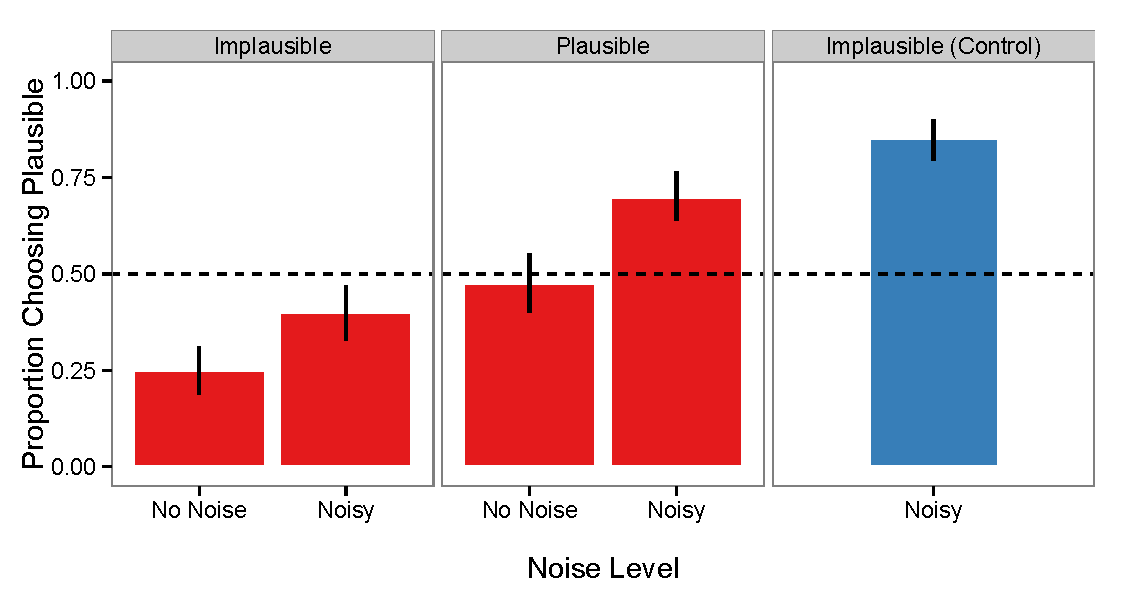
\includegraphics[width=.95\textwidth]{figures/exp2_results.pdf}
    \caption{Experiment 2 Test trial responses. Replicating Experiment 1, 4- and 5-year-old children were more likely to correct the phonological error during Test trials when they were previously exposed to a Plausible speaker, although 3-year-olds were not. Bars show group-averaged proportion of plausible item selection at Test, error bars show 95\% confidence intervals computed by non-parametric bootstrap at the subject level. The dashed line indicates chance performance.}%
   \label{fig:exp2_results}
\end{figure}

Older children were thus more sensitive to the speaker's utterances on unambiguous Exposure trials, and relied more on their speaker-expectations on ambiguous Test trials. Did older children rely more on their speaker-expectations because they had built stronger expectations on Exposure trial? If so, individual differences in children's performance on Exposure trials should explain away the effect of age on Test trials. In contrast, if the ability to leverage these expectations is improving over development, age should predict additional variance in ambiguous Test trial responses over and above children's responses on Exposure trials.

To answer this question, we fit an additional model including the proportion of Exposure trials on which individual children had selected the plausible referent. We assume that children who more frequently selected the plausible referent in the Plausible referent in the Plausible Speaker condition, or less frequently selected the plausible referent in the Implausible Speaker condition were encoding more information about the Speaker's plausibility ($Test \sim age + condition \cdot Exposure + (1|subj) + (1|item)$.

This model showed a significant effect of Plausible Speaker ($\beta_{Plausible} = 1.92$, $z = 3.39$, $p = .001$), a significant effect of individual differences in Exposure selection ($\beta_{Exposure} = 2.84$, $z = 4.60$, $p < .001$), and a significant interaction between Plausible Speaker and Exposure selection ($\beta_{Plausible \: \cdot \: Exposure} = -3.32$, $z = -3.64$, $p < .001$), but no effect of age ($\beta_{age} = .06$, $z = .56$, $p = .57$). This was true both when all of the children were analyzed, and when only the 4- and 5- year olds were included in the model. Thus, older children's increased use of speaker expectations on ambiguous Test trials appears to be explained by their stronger encoding of Speaker preferences on the unambiguous Exposure trials.

Thus, it appears that older children relied more on speaker expectations because they had formed stronger expectations rather than because they rely on expectations differently. Experiments 1 and 2 thus show that children's reliance on speaker-expectations remains relatively constant across the 3--6 year range, but that their ability to build these expectations improves gradually across development.


\section{Experiment 3}

Experiment 3 tests a second prediction of noisy channel processing: As speech becomes noisier, and thus less reliable, children should rely more on their expectations.

\subsection{Method}

\subsubsection{Participants}

For Experiment 3, children were again recruited from the floor of the San Jose Children's Discovery museum. As 3-year-olds did not perform differently from chance in Experiment 2, we again focused on 4- and 5-year olds. Data from a total of 114 children were collected, 1 of whom was excluded for $<50\%$ exposure to English and 2 of whom were excluded for parent-reported developmental disabilities. As before, children were recruited until at least 20 had been run in each condition. Children's ages and genders were again comparable across conditions (Table~\ref{tab:exp3_demos}).


\begin{table}[tb]
\begin{center}
\begin{tabular}{llllll}
 Speaker Condition & Noise Condition & $N$ & $N$ girls & Mean Age (years) & Age Range\\
  \hline
  Plausible & No Noise & 21 & 8 & 4.89 & 4.00--5.83 \\
  Plausible & Noisy & 26 & 12 & 4.89 & 4.02--5.94 \\
  Implausible & No Noise & 20 & 12 & 4.98 & 4.00--5.83 \\
  Implausible & Noisy & 24 & 11 & 5.01 & 4.01--5.92 \\
  Implausible (Control) & Noisy & 20 & 11 & 4.96 & 4.15--5.91 \\
   \hline
\end{tabular}\end{center}
\vspace{6pt}
\caption{\label{tab:exp3_demos}Demographic information for participants in Experiment 3.}
\end{table}

\subsubsection{Stimuli, Design, \& Procedure}


Stimuli were constructed as in Experiments 1 and 2 with a few small changes. First, one additional Test trial was added to increase power. Second, two versions of each acoustic recording were made. One was recorded in a sound-proof room by a female native English speaker. The second was constructed by convolving each recording with randomly generated Brown noise with an amplitude of .7 using Audacity, producing an average signal-to-noise ratio of -19.5dB. The first was used in the No Noise conditions, the second was used to replicate the two conditions from Experiment 1 as well as for the Control condition.

In addition, because all of the Test trials asked the listener to select the semantically implausible referent, it is possible that exposure to an Implausible speaker induced listeners to select the implausible referent at test generally, independent of their acoustic input.  In Experiment 3, we provide a Control condition in which the Implausible speaker from Exposure asked for the semantically plausible referent at test. If children inferred from the unambiguous Exposure trials that the goal of the game was to pick the ``silly'' referent, they should have continued to select the implausible referent on Test trials. In contrast, if Exposure trials caused them to adjust the relative weights on acoustic information and speaker-expectations, they should instead have selected the plausible referent at test.

\subsection{Results}

As in the previous experiments, we first establish that children understood the task, and encoded the differences between the Plausible and Implausible speakers on Exposure trials ($Exposure \sim condition + (1|subj) + (1|item)$). At each noise level, children in the Plausible speaker condition were more likely to select the plausible referent on Exposure trials than those in the Implausible speaker condition ($\beta_{No Noise} = 6.92$, $z =6.15$, $p < .001$, $d = 7.94$; $\beta_{Noisy} = 4.91$, $z =8.26$, $p < .001$, $d = 4.46$). Further, children in the Implausible Control condition performed no differently from those in the Implausible condition, licensing comparison of their Test trials ($\beta_{Control} = .35$, $z =.81$, $p = .42$, $d = .21$).

Second, we again compared the conditions to each other, fitting a mixed-effects regression predicting choice on Exposure trials from noise level and speaker condition (Implausible, Plausible, Control; $Exposure \sim noise \cdot condition + (1|subj) + (1|item)$). Compared to the Implausible Speaker condition, children exposed to the Plausible Speaker were more likely to pick the plausible referent on Exposure trials ($\beta_{Plausible} = 6.62$, $z = 8.88$, $p <.001$). Children exposed to the Control speaker did not perform differently on Exposure trials from those exposed to the Implausible speaker, as predicted ($\beta_{Control} = .36$,  $z = .83$, $p = .42$). Further, the model showed a marginal effect of Noise level ($\beta_{Noisy} = .86$,  $z = 1.74$, $p = .08$) and a significant interaction between Noise level and Speaker ($\beta_{Plausible \: \cdot \: Noisy} = -1.71$, $z= -2.15$, $p = .03$), indicating that the addition of noise moved children in both conditions closer to chance.

\begin{figure}[tb]
     \centering
     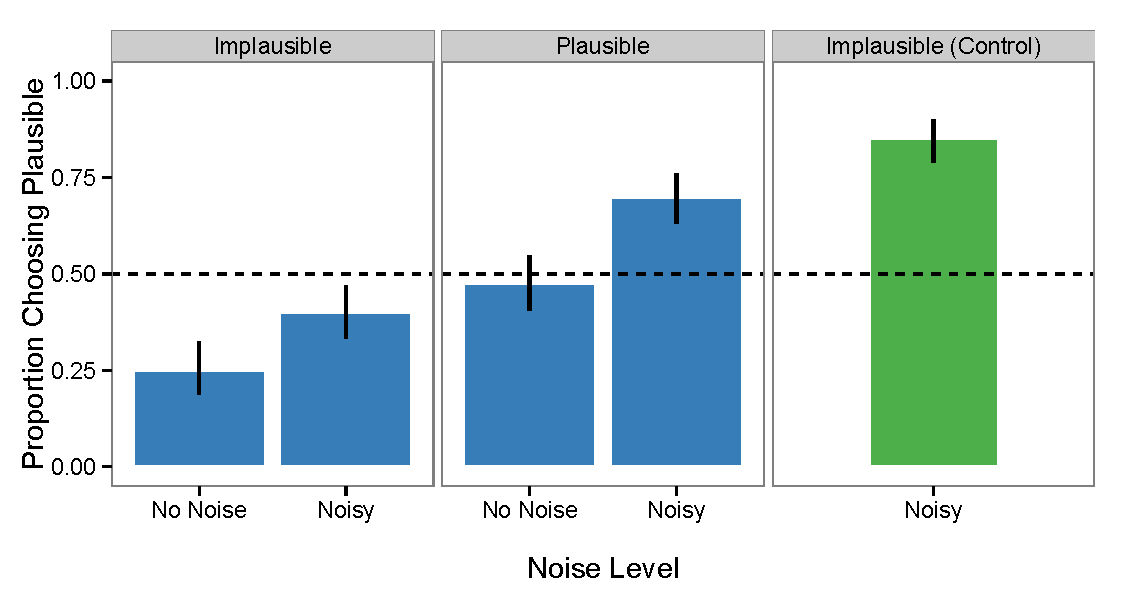
\includegraphics[width=5in]{figures/exp3_results.pdf}
    \caption{Experiment 3 Test trial responses. Replicating Experiments 1 and 2, children were more likely to correct the phonological error during Test trials when they were previously exposed to a Plausible speaker. In addition, in both conditions children were more likely to correct the error when the speech was noisier. Finally, when children were tested in a Control condition, in which a previously Implausible speaker referred to \emph{plausible} referents during ambiguous Test trials, they reliably selected the plausible referent. Together, these results show that children adaptively integrate both bottom-up acoustic information and top-down expectations about the speaker when processing language. Bars show group-averaged proportion of plausible item selection at test, error bars show 95\% confidence intervals computed by non-parametric bootstrap at the subject level. The dashed line indicates chance performance.}%
   \label{fig:exp3_results}
\end{figure}

Did children integrate the noise level of the acoustic stimuli with speaker expectations on the ambiguous Test trials? Figure~\ref{fig:exp3_results} shows the proportion of trials on which children selected the plausible referent at Test in both speaker and noise conditions. As predicted, children showed sensitivity to both speaker reliability and acoustic noise. Children selected the plausible referent at Test, correcting the error in their acoustic input, more often when the speaker had said plausible things on Exposure trials ($Test \sim condition + (1|subj) + (1|item)$; $\beta_{Noisy} = 1.17$, $z =3.72$, $p < .001$, $d = 1.17$; $\beta_{No Noise} = 1.57$, $z = 4.14$, $p < .001$, $d = 1.17$). In addition, regardless of Speaker plausibility, children selected the plausible referent more frequently when the acoustic input was noisy. To quantify this pattern, we again fit a mixed-effects regression predicting choice on test trials from Speaker type and Noise level as well as their interaction ($Test \sim condition \cdot noise + (1|subj) + (1|item)$). As predicted, both main effects were significant ($\beta_{Plausible} = 1.96$,  $z = 3.20$, $p <.001$, $\beta_{Noisy} = .81$,  $z = 2.21$, $p = .03$), but their interaction was not ($\beta_{Plausible \: \cdot \: Noisy} = .33$,  $z = .65$, $p = .51$).

Finally, one alternative explanation for the difference between Speaker conditions is that children simply followed their expectations at all times, e.g., that those exposed to the Implausible speaker chose ``silly'' responses regardless of the question. To test this alternative, we asked whether children who responded to an Implausible speaker on Exposure trials always chose the implausible referent on Test trials even when the speaker referred to the \emph{plausible} referent (Implausible Control condition). A mixed-effects model estimating plausible referent selection on Test trials ($Test \sim condition + (1|subj) + (1|item)$) showed that compared to the Plausible speaker, children exposed to the Implausible speaker were less likely to pick the plausible referent ($\beta_{Implausible} = -1.57$,  $z = -4.14$, $p <.001$; $d = 1.17$), but children in the Control condition were \emph{more} likely to select the plausible referent ($\beta_{Control} = 1.06$,  $z = 2.05$, $p = .04$; $d = 1.93$). Thus, children who were asked for the plausible referent at Test selected it, even when the speaker had previously always referred to the implausible referent. This Control condition provides further evidence that children were attending to and responding to the acoustic input from the speaker on Test trials, integrating it with their prior expectations.


\section{General Discussion}

When we use language to communicate, we are doing more than processing the sounds we hear; we are trying to infer speakers' intended meaning \cite{clark1996}. Because perception is inherently uncertain, our expectations about what speakers are likely to say play an important role in resolving interpretive ambiguities \cite{grice1975, frank2012}. Our experiments show that children are able to integrate speaker expectations with perceptual uncertainty by ages 4--5, though perhaps not earlier. Children's reliance on speaker-expectations appears to track their developing ability to form these expectations, an ability that improves over the preschool years.

In our studies, children adjusted their reliance on expectations as much as adults, but also generally relied more on top-down expectations. Because of the greater noise inherent in children's perceptual processing systems, the same acoustic stimulus may effectively be less reliable for children than adults \cite{neuman1983, lyons2011}. Perhaps children with impaired acoustic processing rely relatively more on their expectations, whereas children with impaired higher-level linguistic expectations rely more on the acoustic signal. Our paradigm could be used to test this prediction.

How much \emph{should} listeners rely on the acoustic signal and how much should they rely on their expectations? Ideal observer models predict that cue should be weighted in proportion to their reliability \cite{jacobs1999, ernst2002}. This prediction holds for adult listeners across levels in language processing from phonology to syntax \cite<e.g.,>{gibson2013, mcclelland2006}. In our experiments, we cannot say that children's weighting was optimal relative to cue reliability, only that it was adaptive: weighting changed with manipulations of reliability \cite<as in>{gibson2013}. It is a challenge for future work to derive independent measures of reliability for high-level linguistic stimuli. Further, because our participants adapted to only one speaker, we cannot know to what extent this adaptation was speaker-specific vs. speaker-general. However, an attractive feature of the noisy channel framework is that it can be applied hierarchically, with appropriate adaptation predicted at the level of speaker, community, and lexicon as evidence accumulates \cite{kleinschmidt2015}.

The results of our experiments show that children, like adults, flexibly trade off between information sources in language comprehension in response to their reliability. Noisy channel principles thus provide a framework for understanding language processing in both adults and children.

%, kleinschmidt2015 and levels

% One puzzle of the broader literature on the development of language comprehension is that children appear to integrate information in an adult-like way in some language processing tasks but not others. A priori, we would predict that children's use of higher-level expectations should be relative to the reliability of their model of the relevant domain. Thus, children should---and do---integrate expectations when the relevant models are over speech sounds, speakers, or semantic plausibility \cite<e.g.,>{clark2009, creel2012, harris2012}. On the other hand, children tend to fail in cases where the relevant models include difficult linguistic content like quantifier semantics or complex syntactic constructions \cite<e.g.,>{trueswell1999, noveck2001}.
% However, based on prior evidence that children's understanding of quantifiers is limited, as is their exposure to relative clauses, this is exactly the result a noisy channel framework for speech processing would predict  \cite{barner2011, montag2015}.
\section{Authorship}
D. Y., S.C., and M.C.F. designed the study. D.Y. and S.C. collected the data. D.Y., S.C., and M.C.F. analyzed the data. D.Y. and M.C.F. wrote the manuscript. All authors approved the final version of the manuscript for submission.

\section{Acknowledgments}

We thank Nicolette Castro, NIH NRSA F32HD075577 to DY, and a John Merck Scholars Fellowship to MCF.

\bibliographystyle{apacite}
\bibliography{noisy_kids}

\end{document}
